%%%%%%%%%%%%%%%%%%%%%%%%%%%%%%%%%%%%%%%%%
% Short Sectioned Assignment
% LaTeX Template
% Version 1.0 (5/5/12)
% This template has been downloaded from:
% http://www.LaTeXTemplates.com
%
% Original author:
% Frits Wenneker (http://www.howtotex.com)
%
% License:
% CC BY-NC-SA 3.0 (http://creativecommons.org/licenses/by-nc-sa/3.0/)
%
%%%%%%%%%%%%%%%%%%%%%%%%%%%%%%%%%%%%%%%%%

%----------------------------------------------------------------------------------------
%	PACKAGES AND OTHER DOCUMENT CONFIGURATIONS
%----------------------------------------------------------------------------------------

\documentclass[paper=a4, parskip=full, fontsize=12pt]{scrartcl} % A4 paper and 12pt font size

\usepackage[]{mcode}
\usepackage[T1]{fontenc} % Use 8-bit encoding that has 256 glyphs
\usepackage{fourier} % Use the Adobe Utopia font for the document - comment this line to return to the LaTeX default
\usepackage[english]{babel} % English language/hyphenation
\usepackage{amsmath,amsfonts,amsthm} % Math packages

\usepackage{lipsum} % Used for inserting dummy 'Lorem ipsum' text into the template

\usepackage{sectsty} % Allows customizing section commands
\allsectionsfont{\centering \normalfont\scshape} % Make all sections centered, the default font and small caps

\usepackage{fancyhdr} % Custom headers and footers
\pagestyle{fancyplain} % Makes all pages in the document conform to the custom headers and footers
\fancyhead{} % No page header - if you want one, create it in the same way as the footers below
\fancyfoot[L]{} % Empty left footer
\fancyfoot[C]{} % Empty center footer
\fancyfoot[C]{\thepage/\pageref{LastPage}} % Page numbering for right footer

\renewcommand{\headrulewidth}{0pt} % Remove header underlines
\renewcommand{\footrulewidth}{0pt} % Remove footer underlines
\setlength{\headheight}{13.6pt} % Customize the height of the header

\numberwithin{equation}{section} % Number equations within sections (i.e. 1.1, 1.2, 2.1, 2.2 instead of 1, 2, 3, 4)
\numberwithin{figure}{section} % Number figures within sections (i.e. 1.1, 1.2, 2.1, 2.2 instead of 1, 2, 3, 4)
\numberwithin{table}{section} % Number tables within sections (i.e. 1.1, 1.2, 2.1, 2.2 instead of 1, 2, 3, 4)

%\setlength\parindent{0pt} % Removes all indentation from paragraphs - comment this line for an assignment with lots of text

% Packages added by JP
% --------------------
\usepackage[]{mcode} % To insert MATLAB codes

\usepackage{lastpage} % To number pages with the format 1/4,2/4,3/4, and 4/4.
\makeatletter
\renewcommand{\@oddfoot}{\hfil \thepage/\pageref{LastPage} \hfil}
\makeatother

\usepackage{graphicx} % Graphicx and subplots
\usepackage{subfig}

\addto\captionsenglish{\renewcommand{\figurename}{Figura}} % Spanish name for figures, tables, and appendix
\addto\captionsenglish{\renewcommand{\tablename}{Tabla}}
\addto\captionsenglish{\renewcommand{\appendixname}{Ap\'endice}}

\usepackage[margin=1.0in]{geometry} % Set all margins to X in/cm

\usepackage{indentfirst} % Indent after the section name
\usepackage{parskip}
\setlength{\parindent}{1cm}

\usepackage[header,title,titletoc]{appendix} % Including the appendix




%----------------------------------------------------------------------------------------
%	TITLE SECTION
%----------------------------------------------------------------------------------------

\newcommand{\horrule}[1]{\rule{\linewidth}{#1}} % Create horizontal rule command with 1 argument of height

\title{	
\normalfont \normalsize
%\textsc{Universidad Yachay Tech, Escuela de Ciencias Matem\'aticas e Inform\'aticas} \\ [15pt] % Your university, school and/or department name(s)
\horrule{0.5pt} \\[0.4cm] % Thin top horizontal rule
\huge Taller 6: Diferenciaci\'on e Integraci\'on Num\'erica \\ % The assignment title
\horrule{2pt} \\[0.5cm] % Thick bottom horizontal rule
}

\author{Valentina Cordova \thanks{\texttt{airina.cordova@yachaytech.edu.ec}} \and Emil Vega\thanks{\texttt{emil.vega@yachaytech.edu.ec}} }  % Your name

\date{\normalsize 7 julio del 2016} % Today's date or a custom date

\begin{document}

\maketitle % Print the title


%----------------------------------------------------------------------------------------
%	PROBLEM 1
%----------------------------------------------------------------------------------------


%------------------------------------------------


\section{Resumen}
\subsection{M\'ETODO DE DIFERENCIAS FINITAS}

Es un m\'etodo que permite la resoluci\'on aproximada de ecuaciones diferenciales en derivadas parciales definidas en recintos finitos. Su expresi\'on matem\'atica esta dada de la forma $f(x+b) - f(x+a)$ que al dividirse por $b-a$ da como resultado un cociente diferencial, que se distingue porque se utilizan cantidades finitas en un lugar de infinitesimales (Boole, 1872). Se consideran normalmente tres formas que son las siguientes: \\

\textbf{Diferencias adelanta}\\
\begin{equation}
{ \Delta  }_{ h }f\left( x \right) =\quad f(x+h)-f(x)
\end{equation}\\

\textbf{Diferencias atrasada}\\
\begin{equation}
\bigtriangledown_{h} f(x)= f(x)-f(x-h)
\end{equation}\\

\textbf{Diferencias centrada}\\
\begin{equation}
\delta _{h} f(x)= f(x+\frac{1}{2}h)- f(x-\frac{1}{2}h))
\end{equation}\\

\subsection{CONCEPTOS ADICIONALES}
\textbf{Condiciones de frontera de Dirichlet}\\
Es un tipo de condici\'on de frontera o contorno, que se utilizan cuando una ecuaci\'on diferencial ordinaria o una en derivadas parciales, se le especifican los valores de la soluci\'on que necesita la frontera del dominio. \\

\textbf{Matriz Tridiagonal}\\
Es una matriz cuyos elementos de su diagonal principal son los \'unicos distintos de cero.\\

\textbf{Orden de convergencia de una soluci\'on num\'erica}\\
Es la velocidad con la cual una sucesi\'on converge a su l\'imite. \\

Finalmente se observa que al utilizar la diferencia centrada con valores de $n$ cada vez mayores, m\'as se acerca la $u$ aproximada a la $u$ real, es decir la soluci\'on discretizada de la ecuaci\'on diferencial con las condiciones iniciales planteadas, se acerca m\'as a la soluci\'on an\'alitica.  

\section{PLANTEAMIENTO DEL PROBLEMA}
\subsection{EJERCICIO 1: Algoritmo en MATLAB}

Cree un m-archivo con el nombre $cds$ que calcule una soluci\'on aproximada para la ecuaci\'on unidimensional estacionaria de convecci\'on-difusi\'on.\\

\begin{equation}
\frac { du }{ dx } =\frac { 1 }{ 50 } \frac { { d }^{ 2 }u }{ d{ x }^{ 2 } }
\end{equation}
con condiciones de Dirichlet $u(0) y u(1)=1$, utilizando el esquema centras de diferencias finitas de la Ecuaci\'on $N° 3$ sobre $n$ nodos equidistantes en el intervalo $[0,1]$ dados por $x_i=(i-1)h$ 
con $\\ h=\frac { 1 }{ n-1 }$ para $i= 1,2,...,n$.\\

En el ejercicio se crea un m-archivo haciendo uso de matlab llamado $cds_EV$ que calcula la soluci\'on aproximada para la ecuaci\'on unidimensional.\\

\subsection{EJERCICIO 2: Soluci\'a anal\'itica y discreta para la ecuación de convecci\'on-difusi\'on}

\textbf{a} Verifique que la soluci\'on anal\'itica de (1) es:

\[u(x)=\frac { exp(50)x -1}{ exp(50)-1}\]


\textbf{b} Verifique que la soluci\'on discreta de (1) mediante el esquema central en diferencias finitas satisface el siguiente sistema de ecuaciones lineales:\\
\[\begin{matrix}
\underbrace { \begin{pmatrix} \beta  & \gamma  &  &  &  &  \\ \alpha  & \beta  & \gamma  &  &  &  \\  & \alpha  & \beta  & \gamma  &  &  \\  &  & \alpha  & \beta  & \gamma  &  \\  &  &  & \alpha  & \beta  & \gamma  \\  &  &  &  & \alpha  & \beta  \end{pmatrix} }_{ A } \underbrace { \begin{pmatrix} { u }_{ 2 } \\ { u }_{ 3 } \\ { u }_{ 4 } \\  \\ { u }_{ n-2 } \\ { u }_{ n-1 } \end{pmatrix} }_{ \tilde { u }  } =\underbrace { \begin{pmatrix} 0 \\ 0 \\ 0 \\  \\  \\ -\gamma  \end{pmatrix} }_{ b } 
\end{matrix}\]\\

\textbf{Donde los coeficientes de A y el vector b est\'an dados por:}\\
$alpha$=$1+25h$\\$beta$= $-2$ \\ y $gamma=1-25h$. \\ El valor de $u_i$ para $i=2,3,4,...,n-2,n-1$ en el vector de inc\'ognitas. Adem\'as $\tilde { u }$ representa la aproximaci\'on de $u(x_i)$. 

\subsection{EJERCICIO 3. An\'alisis del error de discretizaci\'on}

\textbf{a} Graficar $(2)$ y $\tilde { u }$ sobre los nodos  $\{ \left( x\_ i,) \right\} \begin{matrix} n=1 \\ i=2 \end{matrix}$ para $n$ = 11,21,41,81. \\
\textbf{b} Estime el orden de convergencia de la soluci\'on num\'erica en las normas infinito y ${ \left\| \cdot  \right\|  }_{ p(0,1) }$ con $p=1,2$ para $n=161,321,641,1281$.\\

\textbf{Usando la siguiente f\'ormula:}
\begin{equation}
{ \left\| f \right\|  }_{ p(0,1) }\cong { (\int _{ 0 }^{ 1 }{ { \left| f(x) \right|  }^{ P }dx) }  }^{ \frac { 1 }{ P }  }
\end{equation}

\section{METODOLOG\'IA}

\subsection{Descripci\'on de los m\'etodos num\'ericos utilizados y sus respectivas implementaciones computacionales}

\subsection*{EJERCICIO 1}

\textbf{cds\_EV}: Es el algoritmo creado y utilizado para que calcule la soluci\'on aproximada para la ecuaci\'on 4.\\

\subsection*{EJERCICIO 2}
\textbf{a. Verificaci\'on de soluci\'on anal\'itica de (1)}\\

Haciendo uso del comando de $Matlab$ llamado $dsolve$ se confirma que $u(x)=\frac { exp(50)x -1}{ exp(50)-1}$ es soluci\'on de la ecuaci\'on N°4.\\

\textbf{b. Verificaci\'on de soluci\'on discreta de (1)utilizando el esquema central de diferencias finitas}\\

	\textbf{Se utiliza lo siguiente:} con el objetivo de hallar una ecuaci\'on general que se pueda aplicar desde $x_2 hasta x(n-1)$
	
	*$f(x)\cong \frac{(x+h)-(x-h))}{2h}$ (Ecuaci\'on N°3).\\
	
	*$f''(x)\cong \frac{(x+h)+2f(x)+(x-h))}{h^2}$ (Segunda derivada de la Ecuaci\'on N°3)\\
	
		
\textbf{a. Graficar $(2)$  y $\tilde { u }$ }\\

	\textbf{Uso de MATLAB} para gr\'aficar uso el comando $"plot"$ y uso las herramientas para que aparezca las cuatros gr\'aficas que corresponden a los nodos:\\
		
Utilizando el algoritmo $cds\_EV$ y los nodos $xx=[x_2,...,x_(n-1)]$. Se plotea $u=f(xx)$ que es la soluci\'on exacta, y $\tilde { u }$ en nuestro algoritmo es $up$ que es la soluci\'on aproximada de Ecuaci\'on 1 para los mismos valores de $n$. \\ 
\subsection{Listado de los m-archivos realizados:}

\textbf{Ejercicio 1:}\\
* $cds_EV.m$\\
\textbf{Ejercicio 2:}\\
* $eval_fun.m$\\
* $T6_ejercicio2.m$\\
\textbf{Ejercicio 3:}\\
* $T6_ejercicio3_a.m$

	
\footnote{emil.vega@yachaytech.edu.ec\\airina.cordova@yachaytech.edu.ec}

\section{DISCUSI\'ON DE RESULTADOS}\label{sect_result}

\textbf{EJERCICIO 1:}
Para este ejercicio se utiliza el algoritmo llamado $cds\_EV.m$ el cual se denomina en $Matlab$\[function [x,u,xx]=cds_EV(n)\] para el cual el par\'ametro de entrada era $n$ (nodos) que arrojar\'a la soluci\'on de la ecuaci\'on diferencial.\\

\textbf{EJERCICIO 2:} \\
\textbf*{a} Se puede observar que al aumentar el valor de $n$ la soluci\'on exacta y $\tilde { u }$ que en nuestro caso corresponde a $up$ la solución aproximada, se van acercando cada vez m\'as en sus valores. Esto es por que la primera derivada de $u$ es igual a $\\ \frac { 1 }{ 50 } $ multiplicado por su segunda derivada. Como se muestra a continuaci\'on:
 
\[u(x)=\frac { { e }^{ 50x }-1 }{ { e }^{ 50 }-1 }\] 

$u'(x)=\frac { 1 }{ ({ e }^{ 50 }(-1)) } ({ e }^{ 50x }(50))$ Primera derivada de $u$\\

$u''(x)=\frac { 1 }{ { e }^{ 50 }-1 } ({ e }^{ 50x }(50)^{ 2 })$ Segunda derivada de $u$\\
 
$u'=\frac { 1 }{ 50 } u''$ ( Ecuaci\'on 2.1 en cual se reemplaza $u' y u''$)\\ 

->> $\frac { 50{ e }^{ 50x } }{ { e }^{ 50 }-1 } =\frac { 1 }{ 50 } \frac { (50)^{ 2 }{ e }^{ 50x } }{ ({ e }^{ 50 }-1) } $\\

->>$\frac { 50{ e }^{ 50x } }{ { e }^{ 50 }-1 } =\frac { 50{ e }^{ 50x } }{ ({ e }^{ 50 }-1) }$ (Se encuentra la igualdad). \\

Por lo tanto se puede decir anal\'iticamente que $u$ es soluci\'on de la ecuaci\'on diferencial es decir la Ecuaci\'on N°1.

\textbf{b} 

Mediante el an\'alisis hecho en clase, a partir de la siguiente deducci\'on utilizando las Ecuaci\'on 3 y su segunda derivada $f''(x)$ se obtuvo:

1) Se hace un cambio de variable $x_{i}=u_{i}$ y  se tiene:
\begin{center}
$x_{2}=u'_{2}=\frac{u_{3}-u_{1}}{2h}$; $u''_{2}=\frac{1}{50}\frac{u_{3}-2u_{2}+u_{1}}{h^{2}}$
\end{center}
\begin{center}
$\Rightarrow\left( \frac{1}{2h}-\frac{1}{50h^{2}}\right)u_{3}-\left(\frac{1}{2h}+\frac{1}{50h^{2}}\right)u_{1}=0$
\end{center}
\begin{center}
$\Rightarrow\frac{(25h-1)}{50h^{2}}u_{3}+\frac{2u_{2}}{50h^{2}}=0$
\end{center}
\begin{center}
$\boxed{{2u_{2}+(25h-1)u_{3}=0}}$
\end{center}
\begin{center}
$x_{3}=\frac{u_{4}-U_{1}}{2h}=\frac{1}{50}(u_{4}-2u_{3}+u_{2})$
\end{center}
\begin{center}
$\Rightarrow\left(\frac{1}{2h}-\frac{1}{50h^{2}}\right)u-{4}-\left(\frac{1}{2h}-\frac{1}{50h^{2}}\right)u-{2}+\frac{2}{50h_{2}}u-{4}$
\end{center}
\begin{center}
$\left(\frac{25h^{2}-1h}{50h^{2}}\right)u_{4}-\left(\frac{25h^{2}+1h}{50h^{2}}\right)U_{2}+\frac{1}{25}u_{3}=0$
\end{center}
\begin{center}
$\boxed{-(25h+1)u_{2}+2u_{3}+(25h-1)u_{4}=0}$
\end{center}
\begin{center}
$U_{4}=\frac{u_{5}-u_{3}}{2h}=\frac{1}{50h^{2}}(u_{5}-2u_{4}+u_{3})$
\end{center}
\begin{center}
$\boxed{-(25h+1)u_{3}+2u_{4}+(25h-1)u_{5}=0}$
\end{center}
\

Generalizando:
\begin{center}
$\underbrace{-(25h+1)}_{\alpha}U_{2}+\underbrace{2}_{\beta}U_{3}+\underbrace{25h-1)}_{\gamma}U_{4}=0$
\end{center}

\begin{center}
$\alpha U_{3}+\beta U_{4}+\gamma U_{5}=0$
\end{center}

\begin{center}
$\alpha U_{4}+\beta U_{5}+\gamma U_{6}=0$
\end{center}

\begin{center}
$\vdots$
\end{center}

\begin{center}
$\alpha u_{n-3}+\beta U_{n-2}+\gamma u_{n-1}=0$
\end{center}

\begin{center}
$\alpha u_{n-2}+\beta u_{n-}+\gamma u_{n}=0$
\end{center}

\begin{center}
$\alpha u_{n-2}+\beta u_{n-1}\qquad=-\gamma$
\end{center}
\

Adem\'as para ilustrar se toma un valor de $n$ arbitrario para visualizar los resultados que pueden ser obtenidos despu\'es de hallar la ecuaci\'on generalizada anteriormente descrita:\\

$Para\quad n=5\\ A=\quad \begin{pmatrix} 2.00 & 5.25 & 0 \\ -7.25 & 2.00 & 5.25 \\ 0 & -7.25\quad  & 2.00 \end{pmatrix}\quad ;\quad x=\begin{pmatrix} 0 \\ 0,25 \\ 0,50 \\ 0,75 \\ 1,00 \end{pmatrix}\quad ;\quad u=\begin{pmatrix} -0.9030 \\ 0.3440 \\ -1.3708 \end{pmatrix};\quad xx=\begin{pmatrix} 0.25 \\ 0.50 \\ 0.75 \end{pmatrix}$


\textbf{EJERCICIO 3:}

\textbf{a} A continuaci\'on se muestran las cuatro gr\'aficas o figuras que se obtuvieron para cada uno de los $n$.\\

\begin{figure}[hbtp]
\centering
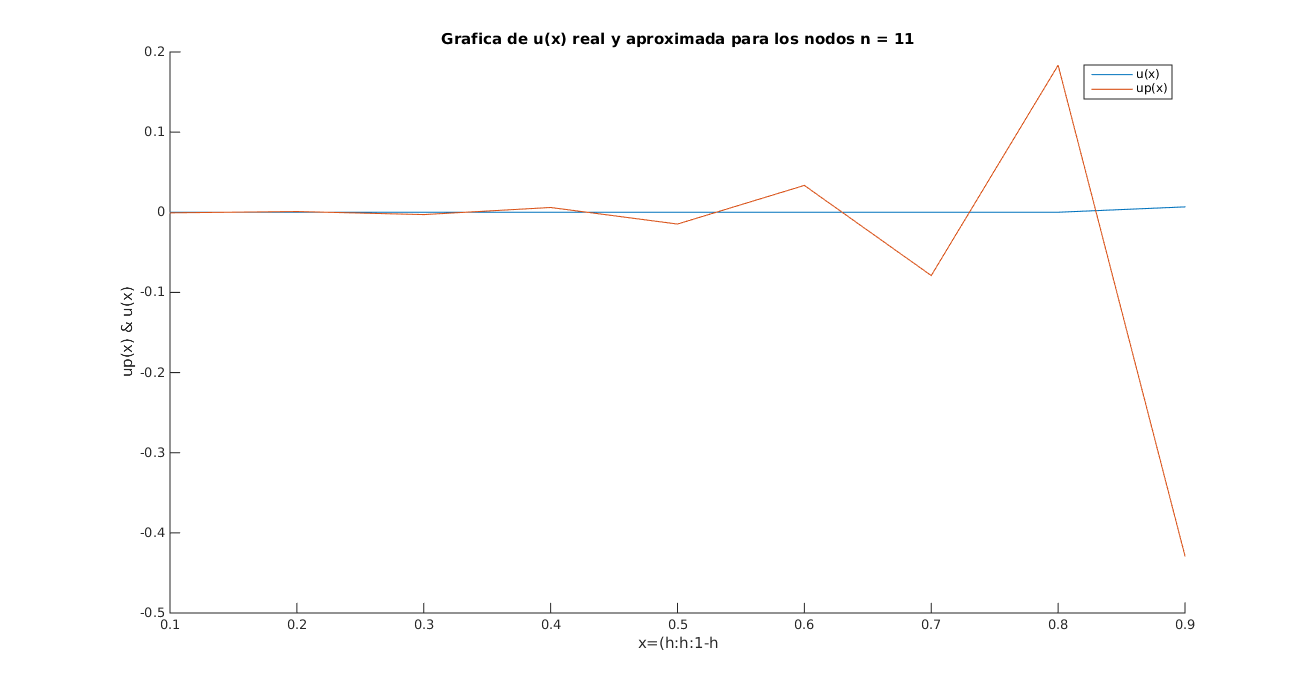
\includegraphics[width=15cm,height=10cm]{n_11.png}
\caption{Figura 1  u(x) real, up(x) vs n=11) }
\end{figure}

\begin{figure}[hbtp]
\centering
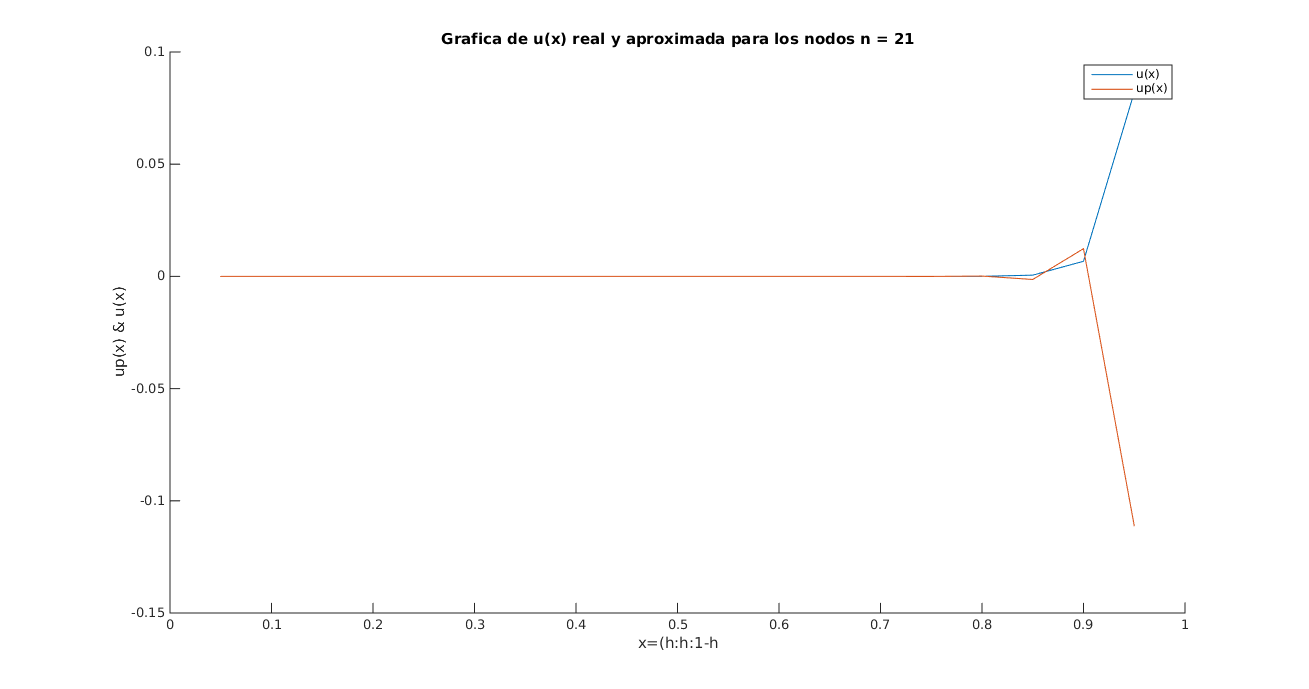
\includegraphics[width=15cm,height=10cm]{n_21.png}
\caption{Figura 2  u(x) real, up(x) vs n=21}
\end{figure}

\begin{figure}[hbtp]
\centering
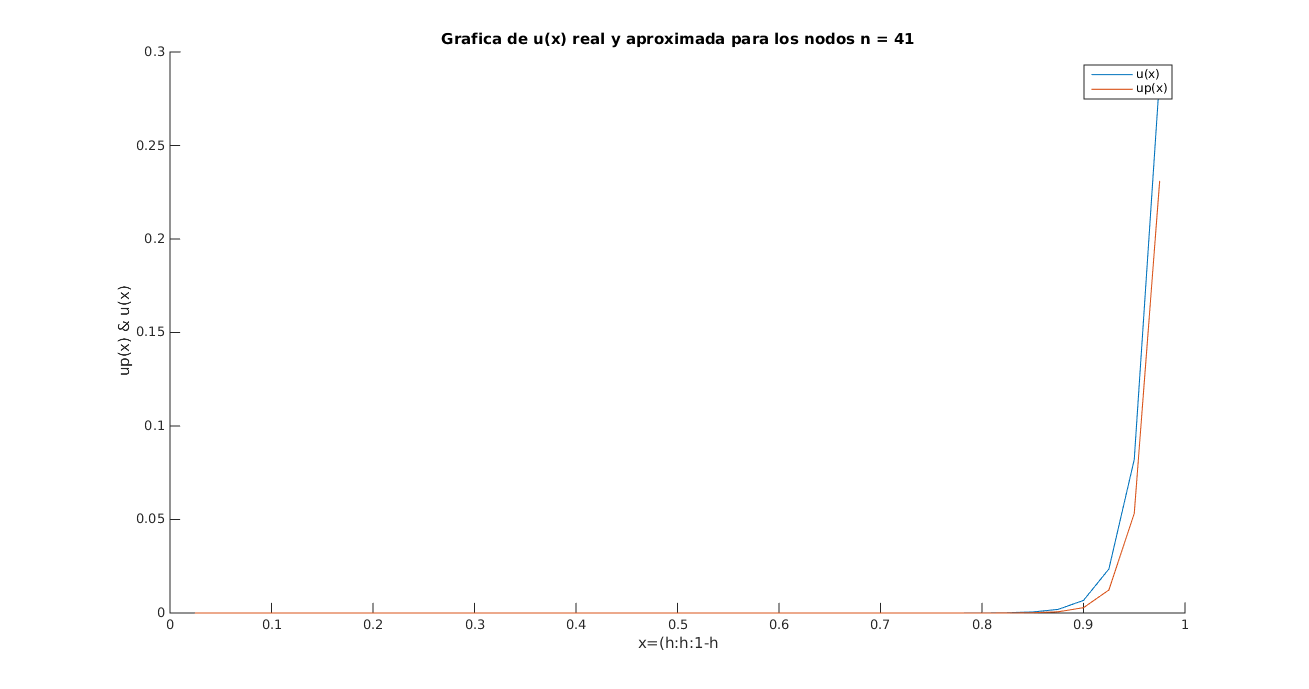
\includegraphics[width=15cm,height=10cm]{n_41.png}
\caption{Figura 3  u(x) real, up(x) vs n=41}
\end{figure}

\begin{figure}[hbtp]
\centering
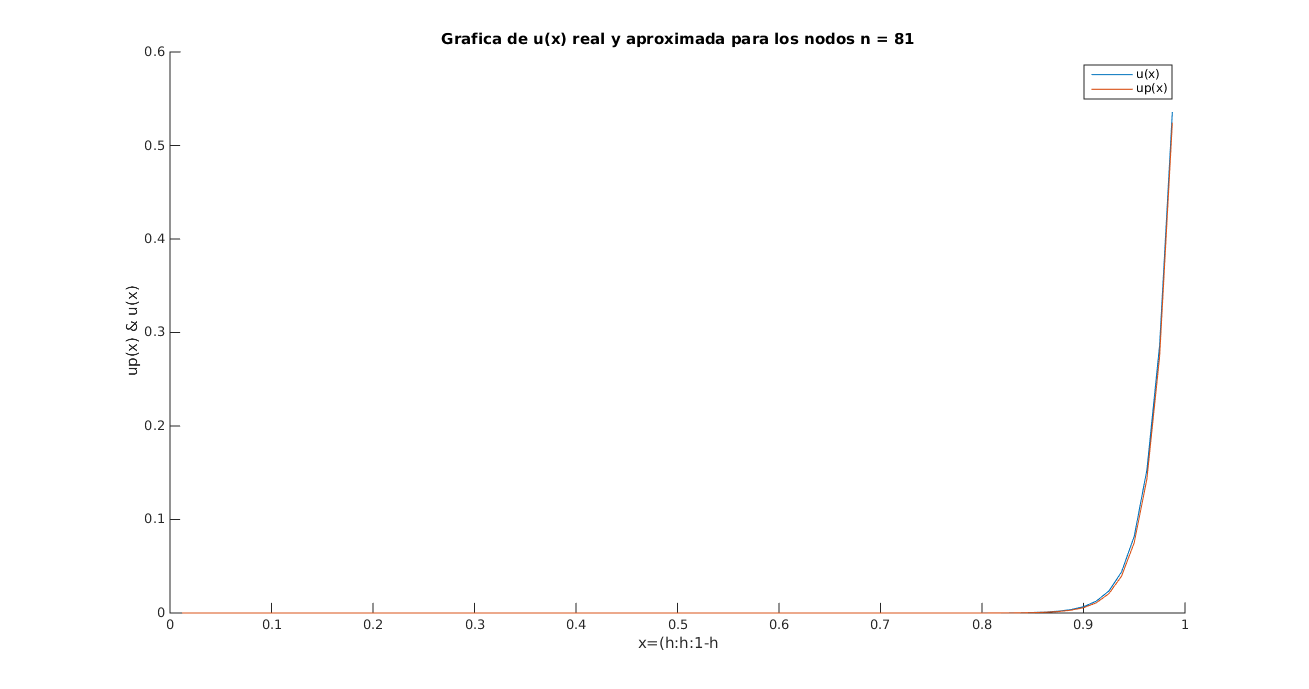
\includegraphics[width=15cm,height=10cm]{n_81.png}
\caption{Figura 4  u(x) real, up(x) vs n=81}
\end{figure}
\
\
\\\\
\\
\\
\\
\\


Al observar la Figura 1, la soluci\'on aproximada est\'a aun muy alejada de la real. Pues las gr\'aficas est\'an bastante separadas una de otras. Cuando comparamos la Figura 1 con la Figura 2 se observa como la $u$ discreta se aproxima un poco m\'as, debido a que $n=21$. Si continuamos con la comparaci\'on, en la Figura 4 la soluci\'on aproximada $up$ está muy junta a la soluci\'on real. Es decir la curva roja está mucho m\'as cerca de la curva de color az\'ul cuando $n=81$. \\


-\textbf{b}: Se encontr\'o la norma infinita y la norma Lp con $p = 1, 2$ para los $n = 161, 321, 641, 1281$ lo cual se muestra en el cuadro 1.
\begin{table}[!htbp]
\centering
\caption{N\'umeros de nodos con sus errores y convergencia}
\begin{tabular}{|c|c|c|c|c|}
\hline 
n & Norma Infinito & Norma Lp ; $p=1$ & Norma Lp ; $p=2$ & Orden de convergencia \\ 
\hline 
161 & 0.003 & 0.00015563 & 0.00056882 & N/A \\ 
\hline 
321 & 0.00074896 & 0.000040122 & 0.00014354 & 1.9557 \\ 
\hline 
641 & 0.00018721 & 0.000010127 & 0.000035942 & 1.9862 \\ 
\hline 
1281 & 0.00004678 & 0.0000025392 & 0.0000089885 & 1.9957 \\ 
\hline 
\end{tabular} 
\end{table}\\
Como se puede observar a medida que se aumentan los nodos, la norma infinito de los errores  como  la norma Lp disminuyen. Adem\'as, si comparamos las normas de los errores entre si, se nota que la norma Lp es menor que la norma infinito. Cabe señalar que los errores para $p=1$ y $p=2$ son muy parecidos. Por lo tanto, en la convergencia para cada nodo se puede ver que se acerca mucho al grado 2 mientras aumentamos los nodos. Esto quiere decir que en el grado $p = 2$ la función converge.

\section{Conclusiones}

\begin{itemize}
    \item Se pudo aprender que la soluci\'on discreta encontrada mediante el esquema central en diferencias finitas, a medida que se aumenta el n\'umero de nodos se aproxima mucho m\'as a la solución anal\'itica, es decir, para obtener la mejor aproximaci\'on, n tiene que ser muy grande.\\
    \item En las Figuras se pudo comprobar de manera visual que si se aumenta el número de nodos, las funciones son similares.\\
    \item Los errores en la norma infinito y Lp disminuyen mientras se aumenta la cantidad de nodos. El error en la norma Lp es menor al error en la norma infinito.\\
    \item El uso de la regla del trapecio compuesto result\'o ser muy \'util y f\'acil de usar para encontrar una aproximaci\'on de la integral para hallar la norma de Lp.\\
\end{itemize}

\section{Referencias Bibliograf\'icas (Opcional)}\label{sect_ref_bib}
Lista de las referencias citadas.

* Cuaderno de M\'etodos Num\'ericos. Cuarto Semestre. Yachay Tech.(2016).
* Granville Sewell, The Numerical Solution of Ordinary and Partial Differential Equations, Academic Press (1988)
* Cheng, A. and D. T. Cheng (2005). Heritage and early history of the boundary element method, Engineering Analysis with Boundary Elements, 29, 268–302.
* Boole, George, A Treatise On The Calculus of Finite Differences, 2ª Ed., Macmillan and Company, 1872.


\newpage

\begin{appendices}
\section{Lista de Programas Computacionales}

\textbf{Ejercicio 1:}
\lstinputlisting{cds_EV.m}


\textbf{Ejercicio 2:}

\lstinputlisting{eval_fun.m}
\textbf{Segundo algoritmo}
\lstinputlisting{T6_ejercicio2.m}

\textbf{Ejercicio 3:}
\textbf{Literal a}
\lstinputlisting{T6_ejercicio3_a.m}

\textbf{Literal b}
\lstinputlisting{T6_ejercicio3_b.m}

\textbf{Orden de Convergencia }
\lstinputlisting{convergencia.m}








\end{appendices}

%----------------------------------------------------------------------------------------

\end{document} 